\documentclass[conference]{IEEEtran}
\IEEEoverridecommandlockouts
% The preceding line is only needed to identify funding in the first footnote. If that is unneeded, please comment it out.

\ifCLASSOPTIONcompsoc
  \usepackage[nocompress]{cite}
\else
  % normal IEEE
  \usepackage{cite}
\fi

\usepackage{caption}
\usepackage{graphicx, subfigure}
\usepackage{algorithm}
\usepackage[noend]{algorithmic}
\usepackage{textcomp}
\usepackage{multirow}
\usepackage{enumitem}

\usepackage{setspace}
\usepackage{amsmath,amssymb,amsfonts}
\def\BibTeX{{\rm B\kern-.05em{\sc i\kern-.025em b}\kern-.08em
    T\kern-.1667em\lower.7ex\hbox{E}\kern-.125emX}}
\renewcommand{\algorithmicrequire}{ \textbf{Input:}} %Use Input in the format of Algorithm
\renewcommand{\algorithmicensure}{ \textbf{Output:}} %UseOutput in the format of Algorithm
%\renewcommand\thesection{\arabic{section}} 
%\renewcommand\thesubsection{\thesection.\Alph{subsection}} 

\begin{document}

\title{Flow-Awareness Maximization by Spatio-Temporal Sampling Collaboration in Software Defined Networks}

\author{He Cai$^{1}$, Jun Deng$^{1}$, Xiaofei Wang$^{1}$
\\
${^1}$Tianjin Key Laboratory of Advanced Networking, %School of Computer Science and Technology,\\
Tianjin University, Tianjin, China.
}


\maketitle

% As a general rule, do not put math, special symbols or citations
% in the abstract
\begin{abstract}
With the proliferation of Internet applications and the explosion of traffic, Fine-gaine's flow-level information acquisition provides basic support for network management, TE, security analysis, and Qos.In traffic sampling, due to the scale of the network, the analysis capcity of the Collector,and the highly dynamic network, there are a large number of flows cannot be captured. In this paper, we focus on maximizing sampling accuracy and sample effective ratio,proposing a collaborative sampling model based on influence, which combines the three dimensional influences of the nodes to quantify the value of the nodes: the direct influence of the current active flow of nodes, the topological influence of the nodes, the historical influence of the nodes; And through the overlapping relationship of active flows between nodes, the cooperative sampling relationship of nodes at sampling timing is constructed. Based on this model, we propose the Agile Flow-Level Co-sampling strategy(AFCS), which solves the approximate optimal solution of CSBI through three steps: sampling point selection, sampling time allocation, and collaborative strategy optimization. We evaluated our strategy through a real large-scale topology, and the results show that it can effectively improve the sampling accuracy, especially in the mice-flow accuracy, and effectively improve the sampling efficiency.
\end{abstract}
%from the three dimensions of sampling node selection, time allocation and collaboration between nodes.
\IEEEpeerreviewmaketitle

\section{Introduction}

With the data traffic and network scale rapidly increasing, flow-level measurement is crucial to network management. In a large-scale network, accuracy is a vital statistic for flow-level sampling. High-accuracy sampling can provide more information for managers and network applications, such as intrusion detection systems(IDS), traffic engineering (TE) and application-aware networks. Especially for network security, over 80% of the flows in the network are mice flows [xx], which have few and scattered packets, making it easier for distributed attacks to hide in them.
These malware propagations via the internet can be prevented by capturing suspicious packets on the network and inspecting them by using security application solutions such as an IDS. Therefore, the higher the sampling accuracy, the higher the network security.
        

We consider two sampling approaches: the systematic packet sampling(SPS) and probabilistic packet sampling(PPS)[xx]. The former approach captures every packet for a sampling duration from a starting point in time. The other is a method to selectively capture packets from flows with a probability. They transmit packets to a unified analyzer (e.g. ,IDS) according to a certain routing rule. 
In a traditional network, there is no flexible way to deal with the changes of real-time traffic because of the closeness and isolation of network.Thanks to the birth of software-defined network. SDN replaces the distributed, per-switch control planes of traditional networks with a (logically) centralized control plane that programs the forwarding behavior of all the switches in a given network. This centralized control plane, run on a controller that gathers traffic and other measurements from the network and uses the gathered information to compute and install forwarding behaviors in the switches. Recur to its centralized control and global visibility,there are more strategies for flow collection on the SDN.SDN controllers can gather traffic of any node with different strategies through a simple OpenFlow [2] protocol, which is incomparable in a traditional network.

When sampling in a large-scale network, in order to reduce the intrusion to the network, it is common to select several nodes to sample in the whole network. 
To maximize the sampling accuracy of flows, many studies have used  social network theory to solve this problem [3,4]. And article [1,5] uses the number of active flows currently  detected by the node  as the influence to quantify the value of the node and select the sampling node.
The sampling rate of nodes is another reason that affects the sampling accuracy. It is limited by constraints, such as the processing capacity of IDS, and is a limited sampling resource.

The Sampling rate of nodes is another reason that affects the sampling accuracy.It is limited by some constraints, such as the processing capacity of IDS ,which is finite resources used for sampling.It is essential to determine a reasonable sampling rate for each node under a given constraint.For example, [3] uses Isometric allocation to determine the sampling rate for each node.Therefore,Selecting the sampling nodes and determining the sampling rate are two important factors that affect the accuracy. 

The validity of sampling that represents the ratio of  redundant samples to all sampled packets,is also a unignorable reason. Redundant packets are generated when a flow passes through multiple nodes at the same time, and at least two nodes capture the same packets from the flow.
The higher the repetition rate,the more meaningless overheads of collector, which may reduce efficiency and even limit sthe promotion of accuracy. 
Therefore, our motivation is to reduce the repetition rate while determining the sampling node and sampling rate,so as to save sampling resources and ultimately maximize the sampling accuracy under the constraint of given collector capacity.

In this paper, we use SPS method.1)When quantifying the node's integrated value, which can be used as a basis to determine the sampling node and sampling time,we consider not only the direct value brought by the current active flow of th node, but also the potential value consisting of the location in a topology and historical vitality of nodes in the sampling period.
2)We first proposed a cooperative sampling strategy among nodes, which considers not only node selection and time allocation, but also the sampling order of nodes in the time dimension for improving the accuracy. With the help of sampling strategy, the sampling order of each node is reasonably arranged in the time dimension,which can reduce the repetition rate markedly and further maintain the accuracy.
3)Therefore, we establish a model to quantify the maximum of  flow-level sampling accuracy, in which  the comprehensive impact of each node is used to evaluate the comprehensive value of the node, and the sampling order is used to optimize the sampling accuracy.
4) Based on the above model, we propose an AFCS strategy, which resolves the overall problem into three solvable sub-problems: node selection, time allocation, and cooperative sampling optimization. AFCS includes three related algorithms: XXX, XXXX, XXX. The output of the previous algorithm is the input to the next algorithm. And finally we obtains the approximate optimal solution of maximizing  sampling accuracy through the heuristics method.


\subsection{Related Work}

\subsection{Contributions}

Our main contributions are summarized as follows:
\begin{itemize}[leftmargin=*]
\setlength{\parindent}{0pt}

\item In the context of Flow-level traffic sampling, we first proposed the concept of cooperative sampling, and explained the effect of timing cooperation between nodes on sampling accuracy and sampling efficiency.
\item For the first time, we modeled the problem of maximizing flow sampling accuracy. It constructs the cooperative relationship of the nodes through the overlapping relationship between the nodes, and quantifies the value of the nodes in the sampling period through the three dimensions of the node's current value, topological value and historical value.
\item Based on this model, we propose an AFCS strategy for solving the approximate optimal solution of the model. The strategy consists of three algorithms: \textbf{Iterative comprehensive influence-based $Top-K$ node selection based on flow privatization}, \textbf{Non-starved influence change-aware priority polling slot allocation}, \textbf{Co-Sampling slots ordering based on effectiveness maximizing greed}.And, We evaluated it through a real large-scale network topology.
\end{itemize}

\begin{figure}[!hhhhhhhhhht]
\centering
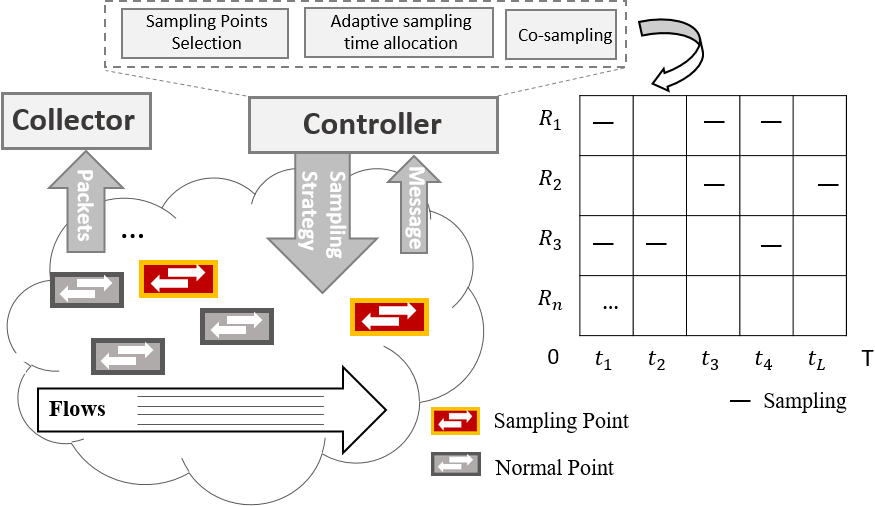
\includegraphics[width=8.5cm]{images/png_architecture.png}
\caption{Co-Sampling Architecture}
\label{Architecture}
\end{figure}




\section{SYSTEM DESCRIPTION AND PROBLEM STATEMENT }

Figure \ref{Architecture} briefly demonstrates the process of node cooperative sampling with AFCS under two constraints: the collector capability $C packets/T$ and the number of sampling nodes $K$. 
Before a new sampling period $T$ begins, in order to maximize sampling accuracy over $T$, each node is assigned a different number of sampling time slots and is arranged slot sequence at the same time.
And all the sampling nodes work together to maximize the sampling accuracy of the flow. %(采样精度 名词需要在引言中解释)all the nodes work together to maximize the sampling accuracy of the flow.
\subsection{Factors affecting sampling accuracy}
In a large-scale network, the challenges to maximize the flow-level sampling accuracy are how to select $K$ sampling nodes and how to allocate sampling time for these nodes over $T$ without exceeding the constraints of $C$ and $K$ values.  %(不超过K值的约束,偏偏又选出K个节点,意思在明确一下)
For node selection and time allocation, we should  consider not only the current detected flow information, but also the possibility of new flow arriving at each node during a $T$ cycle after running the sampling strategy. %(其实我一直想知道用这种简写T 用不用再加上其他修饰词 比如 a the 比如 cycle time)
In addition, another important factor affecting the sampling accuracy is the repetition rate of the sampled packets, which represents the ratio of the repeated packets to all the packets.
Collecting repeated packets not only occupies limited resources and reduces the sampling validity, but also reduces the  accuracy.  %(validity 常用于表示数据有效性)
The higher the repetition rate, the more meaningless  overheads of collector, which may limit the promotion of sampling accuracy or even reduce accuracy. %(跟上面的句子有点冗余了)
%Therefore, in order to improve the flow-level sampling accuracy , we need to focus on three aspects: node selection, time allocation and reducing unnecessary repetition rate. %(建议把flow-level sampling accuracy 进行字母缩写)

Repeated packets are generated when a data flow passes through multiple nodes at the same time, and at least two nodes capture the same packets from the flow. %(are generated when 这种语法需要确认)
That is to say, \emph{the overlap of the flows covered by nodes and the arrangement of sampling time sequence among nodes determine the repetition rate}.The overlapping relationship of the flows covered by the nodes and the overlapping relationship of the nodes in the sampling time dimension directly determine the repetition rate.
To a certain extent, reducing unnecessary repetition rate is conducive to improving accuracy.
From this perspective, in an optimal model, the overlap of flow among nodes, the order of nodes in the  dimension of a cycle time, the value brought by the order of nodes, should be integrated into the node selection and time allocation. 
Since the goal of the system is to give priority to maximizing sampling accuracy, sometimes the repetition rate is unavoidable. And the repetition rate is necessary, if the value brought by it can maximize the sampling accuracy.

\subsection{PROBLEM Model}
Maximizing sampling accuracy of flows is the same as maximizing area coverage, as shown in Figure \ref{fig_1_model}.
The red solid area represents all flows passing through the whole network during the $T$, including currently active flows and subsequently arrive flows,denoted as $F^c$.The gray area is the set of active flows currently passing through the node, denoted as $F_i^c$, and the red area is the set of flows that the node may newly arrive in within T.
When maximizing the area coverage, the gray area of the node and the red dotted area should be fully calculated. And the overlap of the areas between the nodes should also be considered,which is regarded as flow overlap mentioned above.
For the value generated by the node, we should not only consider the value brought by its current flows(\textbf{Direct Value}), but also the value brought by the new arrival flows in T(\textbf{Potential Value}).The area coverage problem is like a traditional sampling solution, a two-dimensional problem: only consider selecting nodes and allocating sampling time. However, the effect of the overlap of flows between nodes on the sampling accuracy in the time dimension is not considered.
\begin{figure}[!!!!!!!!!!!!!!hhhhhhhhhht]
\centering

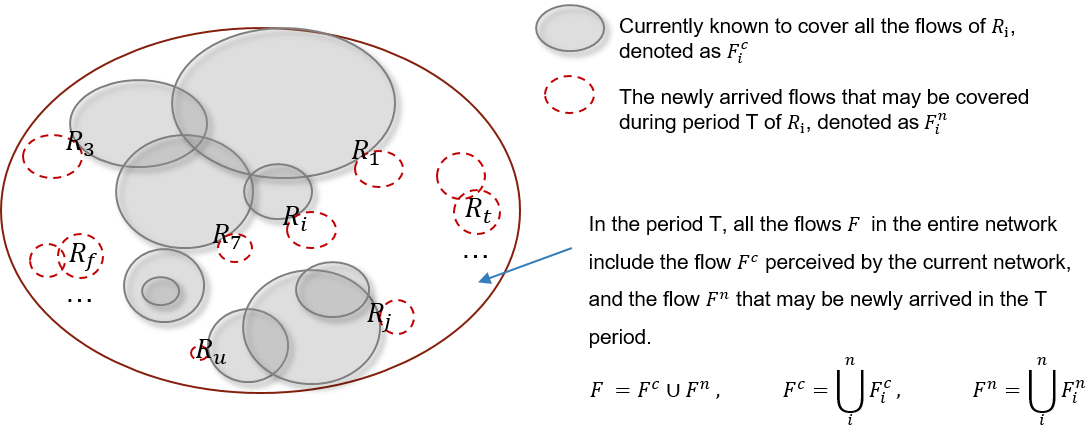
\includegraphics[width=7cm]{images/area_coverage.png}
\label{fig_1_area}

\caption{Area coverage problem}
\label{fig_1_model}
\end{figure}

In order to establish a model to maximize the sampling accuracy of flows, it is necessary to quantify the value and the cost of each node, based on the overlap of flows and the cooperation strategy in the time dimension.Let $R$ as the set of all nodes.
%We consider the size of the set $F^c_i$ consisting of flows $f_k$ captured by the node as the direct value of the $i_{th}$ node $R_i$.
For any $f_k$ in the set $F^c_i$, if any packet of $f_k$ is captured by $R_i$, and then $f_k$ is considered to be successfully captured by $R_i$.
Assuming that the arrival of packets of a flow $f_k$ obeys the poisson distribution with ${\lambda_{k}}$ during the unit time $t$,then the expected number of current active flows captured by $R_i$ is $\sum_{f_k \in F^c_i}{P\{N_p^k(t) > 0\}}$.
Therefore, we can easily quantify the direct value that the node brings in $t$.
But for the potential value of nodes, we do not know the number of flows that will arrive at each node during a T in the future. Even the arrival distribution of flows is known,, we can not know the overlap of these flows among the nodes. Therefore, the potential value of nodes needs an independent quantification method.(independent to other nodes).

We propose a quantification approach based on comprehensive influence, which unifies direct value and potential value.
Let $t$ is the unit time, $t$ is the smallest unit of sampling duration allocation, $t<=T$. And let $L = T/t$ represents the number of time slots.
The direct influence of any node $R_i$ within a $t$ can be quantified as (\ref{model_di}).
It is described as the expected number of currently active flows captured by the node within $t$ divided by the total number of currently active flows of whole network.
The quantization method is based on the flow betweenness centrality(FBC)[2], which reflects the timely influence of nodes.
\begin{equation}
D_i= \sum\limits_{{{f}_{k}}\in {{F}^{c}}}{P\left\{ N_{p}^{k}\left( t \right)>0 \right\}} /|F^c|
\label{model_di}
\end{equation}
And we evaluate the potential value of nodes from two dimensions: the power of the node in the network topology,and the proportion of the number of previous flows.
We use standard betweenness centrality to measure the power of node $R_i$ in the network[2], which we call the topology influence of nodes $S_i$ and which represents the importance of the location in the network topology.
The proportion of the number of previous flows reflects the activity of the node throughout the network lifecycle, called history influence $H_i$. 
$H_i=TF_i/TF$,where $TF_i$ represents the number of flows that has passed $R_i$ so far, and $TF$ is the total number of flows that have passed the network so far.

Therefore, the potential value of the node during a $T$ can be quantified using $S_i$ and $H_i$.The higher the $S_i$ and $H_i$, the higher their potential value and the more likely they are to go through more flows in the future.
And during a $t$,the compositive value generated by the node can be expressed as $\alpha \cdot D_i +  \beta \cdot \frac{S_i}{L} + \gamma \cdot \frac{H_i}{L}$, where $\alpha + \beta + \gamma =1$ represents the weighted sum of the three influences.%$\frac{1}{L}$ represents the potential influence in t.

The cost of $R_i$ is the total number of packets collected in unit time.
We use $w_i$ to represent the total number of packets detected by $R_i$ within $t$. %介词
 $w_i$ can be expressed as (\ref{wi}), where $v_i$ is the current packet rate $(packets/T)$ of $R_i$. Because of the subsequent arrival of unknown traffic, we use the ratio of potential value to direct value to infer $w_i$.
\begin{equation}
{{w}_{i}}= \frac{1}{L} \cdot [v_i + v_i \cdot \frac{\beta \cdot \frac{S_i}{L} + \gamma \cdot \frac{H_i}{L}}{\alpha \cdot D_i}]
\label{wi}
\end{equation}
We give the Influence-based maximization flow sampling accuracy collaborative sampling model in (\ref{1}), where ${{s}^{l}}($l=1,2...,L$)$ represents the different $t$ slots in T. (\ref{2}) (\ref{3}) describe the constraints that the model should satisfy. 
\begin{spacing}{0.5}
\begin{small}
\begin{equation}
\begin{split}
%\begin{gather}
\max \sum\limits_{i}^{n}{(\alpha \cdot {\delta ({{D}_{i}},\left| \widetilde{{{S}_{i}}} \right|)}+\frac{\left| \widetilde{{{S}_{i}}} \right|}{L\;}\cdot (\beta \cdot {{S}_{i}}+\gamma \cdot {{H}_{i}}))} 
- IR \label{1}
%\end{gather}
\end{split}
\end{equation}

\begin{equation}
subject \ to: \sum\nolimits_i^n {f(\widetilde {{S_i}}) \le } K,f(\widetilde {{S_i}}) = \left\{ \begin{array}{l}
1,\left| {\widetilde {{S_i}}} \right| \ge 1\\
0,\left| {\widetilde {{S_i}}} \right| = 0
\end{array} \right.\label{2}
\end{equation}
\begin{equation}
\sum\nolimits_{i}^{n}{{{w}_{i}}\cdot \left| \widetilde{{{S}_{i}}} \right|\le C}\label{3}
\end{equation}
\end{small}
\end{spacing}
\vskip 0.2 cm

The goal of the model is to allocate the corresponding sampling time for each $R_i$ under the constraints of given $C$ and $K$, and to determine the sampling cooperation strategy among nodes, when maximizing the influence of the system in the period $T$ or maximizing the flow-level sampling accuracy. 
$\widetilde{{{S}_{i}}}$ represents the set of slots allocated to $R_i$. The different slots in
$\widetilde{{{S}_{i}}}$ represent the sampling arrangement of the node in the time dimension. The larger the size $|\widetilde{{{S}_{i}}}|$, the greater the comprehensive influence (value) generated by the node.The relationship between the comprehensive influence of nodes and $|\widetilde{{{S}_{i}}}|$ is given in (\ref{4}).
\begin{equation}
\delta \left( {{v_i},\left| {\widetilde {{S_i}}} \right|} \right) = \left\{ \begin{array}{l}
{v_i} \cdot \left| {\widetilde {{S_i}}} \right|,{\rm{    }}{v_i} \cdot \left| {\widetilde {{S_i}}} \right| < \left| {F_i^c} \right|\\
\left| {F_i^c} \right|{\rm{   }}\quad,\ {\rm{    ELSE}}
\end{array} \right.\label{4}
\end{equation}
When $ D_i\cdot |\widetilde{{{S}_{i}}}|=|F^c_i|$, it means that $R_i$ can capture all the flows of $F^c_i$ under $|\widetilde{{{S}_{i}}}|$ $t$.Then its direct value will not continue to increase with the increase of $|\widetilde{{{S}_{i}}}|$, but the potential value will continue to increase. 
%In addition, when a flow is collected by different nodes in the same slot, the actual number of flow in the whole system does not increase. 
Therefore, the value generated by a single slot of a node is related to the number of slots the node already has, not independent.

In (\ref{1}), the first part represents the sum of the combined values of all nodes under their respective $\widetilde{S}_i$; And the subtraction part $IR$ indicates the sum of the direct influences of the resampled flows at all the same time slots which described in (\ref{ir}), where the $\psi ({{f}_{k}},{{s}^{l}})$
calculates the number of times each flow is resampled at slot $s^l$. $U = \left\{ {{R_i},{f_k} \in F_i^c \wedge {s^l} \in \widetilde {{S_i}}} \right\}$ is a set of routers which contain $f_k$ and sampling at time $s^l$.
 As mentioned above, 
the packet repetition rate is generated by more than one nodes sampling the same flows at the same time.Therefore, the model takes the overlapping relationship of flows between nodes and the arrangement of nodes in the sampling time dimension as one of the factors that influence the accuracy of flow sampling. In order to maximize (1), \emph{each sampling node must have a reasonable slots arrangement for sampling, collaboration of sampling nodes in time dimension, in exchange for the improvement of sampling accuracy.}

\begin{spacing}{0.5}
\begin{small}
\begin{equation}
\begin{split}
%\begin{gather}
IR=\frac{\alpha }{\left| {{F}^{c}} \right|}\cdot \sum\limits_{{{f}_{k}}\in {{F}^{c}}}{\sum\limits_{l=1}^{L\;}{\left( P\left\{ N_{p}^{k}\left( t \right)>0 \right\}\cdot \psi \left( {{f}_{k}},{{s}^{l}} \right) \right)}} \label{ir}
%\end{gather}
\end{split}
\end{equation}
\end{small}

%%%%%
%%%%%%%%%%%%%%%%%%%%%%%%%%%%%%%%%%%%%%%%%%%%%%%%%%%%%

\begin{small}
\begin{equation}
\psi \left( {{f_k},{s^l}} \right) = \left\{ \begin{array}{l}
\left| U \right| - 1,{\rm{    }}\left| U \right| \ge 1\\
{\rm{   }}0\quad \quad \; \; ,\, \left| U \right| = 0
\end{array} \right.\label{5}
\end{equation}
\end{small}
\end{spacing}
\vskip 0.2 cm

We explained the quantization process of the model and illustrated it as Figure\ref{fig_1_model}.The goal of the model is to allocate reasonable $\widetilde{{{S}_{i}}}$ sets for all $R_i$ under constraint conditions.As  figure\ref{fig_1_model} shows, when the system gets the optimal solution of $S ^ 1..S ^ n $, it not only reflects the optimal node selection, the optimal time allocation, but also reflects the optimal slot order arrangement, which is determined by the cooperation strategy between nodes. At the same time, each node actually avoid overlapping on the same slot as much as possible, so that the efficiency of the sampling system is improved. The time complexity for solving this model is $O(2^{|R| \cdot L})$.

 

\begin{figure}[!!!!!!!!!!!!!!hhhhhhhhhht]
\centering

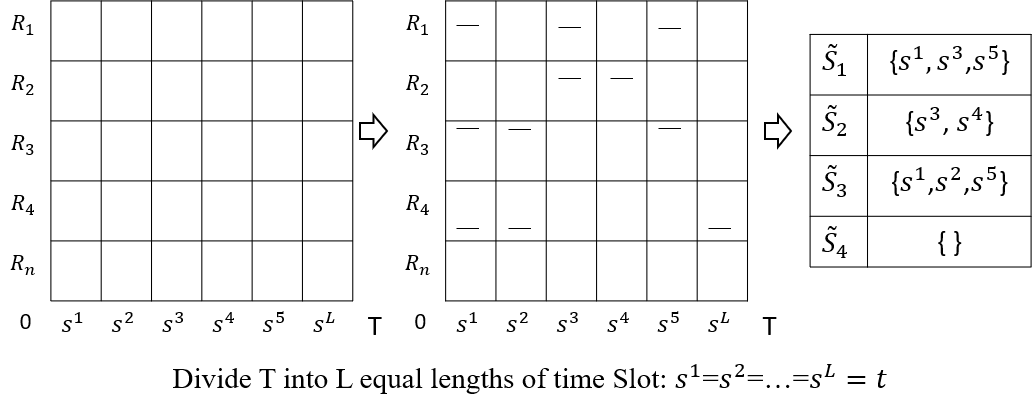
\includegraphics[width=8.5cm]{images/slot_num_order.png}
\label{fig_1_slot}

\caption{Overview of model}
\label{fig_1_model}
\end{figure}



\section{Agile Flow-Level Co-sampling strategy(AFCS)}
Since the above model is complicated, we divide it into three sub-problems: K node selection, Slot allocation, and collaborative sampling optimization. The solution to each sub-question will be the input to the next sub-question. Through three steps, the approximate optimal solution of the total problem is obtained.In this section, we detail each sub-question and propose the corresponding algorithms.

\subsection{Iterative comprehensive influence-based $Top-K$ node selection based on flow privatization} 

In the selection of K sampling points, we only focus how to use the static properties of the nodes to quantify their comprehensive influence, which is independent of time allocation. In (\ref{1}), when the number of slots and the cooperative relationship between nodes (slots order) are not considered, the optimization formula can be expressed as (\ref{maxk}) and the constraint is (\ref{maxkc});The goal of the optimization model (\ref{maxk}) is to select K sampling nodes without considering the influence of time on the comprehensive influence of the nodes, so as to maximize the comprehensive influence of the system.Similar to the model of (\ref{1}), the former part sums the comprehensive influence of the selected nodes, and the latter part subtracts the influence part of the repeated calculations.
\begin{spacing}{0.5}
\begin{small}
\begin{equation}
\max [\sum_{i=1}^n (\alpha \cdot {D_{i}} + \beta \cdot {S_{i}} + \gamma \cdot {H_{i}}) \cdot \varphi{(i)} - \alpha \cdot\sum_{f_k \in F^c} \widehat{\psi}{(f_k)}]
\label{maxk}
\end{equation}
\begin{equation}
subject \ to:\sum_{i=1}^{n} \varphi(i) = K
\label{maxkc}
\end{equation}
\end{small}
\end{spacing}
\vskip 0.2 cm
In(\ref{maxk}), $D_i=|F^c_i|/|F^c|$,and $\varphi(i)$ is 0 means that $R_i$ is not selected, 1 means $R_i$ is selected;$\widehat{U} = \{R_i,f_k \in F^c_i \wedge \varphi(i) = 1\}$ indicates how many selected nodes cover $f_k$,so the(\ref{maxkr}) indicates how many selected nodes are repeatedly calculated $f_k$ as their direct influence.Therefore, the subtracted part expresses that any flow will only be calculated once as a direct influence,in other words, any flow will only be calculated as direct influence by only one of the selected nodes, \emph{the flow is privatized by a selected node during the selection process.}
\vskip 0.2 cm
\begin{spacing}{0.5}
\begin{small}
\begin{equation}
\widehat{\psi} \left( {{f_k}} \right) = \left\{ \begin{array}{l}
\left| \widehat{U} \right| - 1,{\rm{    }}\left| \widehat{U} \right| \ge 1\\
{\rm{   }}0\quad \quad \; \; ,\, \left| \widehat{U} \right| = 0
\end{array} \right.
\label{maxkr}
\end{equation}
\end{small}
\end{spacing}
\vskip 0.2 cm
Therefore, it is possible to iteratively calculate the top $K$ nodes with the most comprehensive influence, the highest comprehensive influence in each round will be selected, and privatize all the flows it covers (but not including the flows privatized by other selected nodes in the previous);That is, for the direct influence of the candidate $R_i$ in the $k$ round, use the flow set $\widetilde{F}^{cs}_i$ to calculate the direct influence; Let $F_k^{cs}$ denote the set of flows privatized by the selected node in the $k_{th}$ round, so $\widetilde{F}^{cs}_i = F_i^c- \bigcup_{m=1}^{k-1}F_m^{cs}$,and the subtracted portion indicates that it has been privatized by the selected node of the previous k-1 round;If $R_i$ is selected in this round, the flows in $\widetilde{F}^{cs}_i$ is $R_i$ exclusive,then $\widetilde{F}^{cs}_i$ written as $F^{cs}_k$,$R_i$ is written as $R^s_k$; In the $k+1$ round selection, even if the other candidate nodes cover these flows, these flows have been privatized by the $R_i$, will not bring value to these candidate nodes in the $k+1$ round. The K-round selection is carried out, and the nodes with the highest comprehensive influence are selected in each round,through the process of privatizing the flows with the most influential nodes in each round, any two selected nodes are: $F^{cs}_i \bigcap F^{cs}_j = \varnothing$, and the comprehensive influence of each node is the highest in the corresponding round, so the K selected nodes guarantee (\ref{maxk}) to be maximized under the constraint (\ref{maxkc}). so the $K$ nodes are the optimal solutions of (\ref{maxk}). $D_i^k$ indicates the direct influence of the candidate node $R_i$ in the $k_{th}$ round selection, which $D_i^k = |\widetilde{F}^{cs}_i|/{\left| F^c \right|}$. (\ref{maxki}) describes the iterative calculation formula for the comprehensive influence of the candidate nodes for each round of selection.
\begin{equation}
I_{i}^{k}=\alpha \cdot D_{i}^{k}+\beta \cdot {{S}_{i}}+\gamma \cdot {{H}_{i}}
\label{maxki}
\end{equation}
Algorithm 1 gives the solution process, and the time complexity of the algorithm is $O(K*|R|)$. % and Fig3 also shows the change process of direct influence in each round of elections.
 Finally, the $K$ node set $R^s$ and the $F^{cs}$ set corresponding to each node can be obtained.


\begin{algorithm}[h]
\caption{Sampling Point Selection}
\begin{algorithmic}[1]

\STATE define $R^s=\varnothing$  //  The Set of Selected Routers

\FOR{$k=1$; $k < K$; $k++$ }

\FOR{each $R_i \in R-R^s$}
\IF{$I_i^k > max$}
\STATE $max = I_i^k$
\STATE $R^s_k = R_i$
\ENDIF
\ENDFOR
\STATE put $R^s_k$ into $R^s$
\STATE $F_K^{cs} = F_i^c- \bigcup_{m=1}^{k-1}F_m^{cs}$ 
\ENDFOR

\RETURN $R^s$
\label{code:recentEnd}
\end{algorithmic}
\end{algorithm}

\subsection{Non-starved influence change-aware priority polling slot allocation}

After the nodes is selected, the number of slots needs to be allocated to these nodes when the constraint (\ref{3}) is satisfied and the slots sequence between nodes is not considered.The optimization model of the subproblem is (\ref{dasd}), which is still judged by formula (\ref{4}).The goal of the model is to maximize system value under the given $R^s$ and constraints (\ref{3}). 
\begin{equation}
\max [ \alpha \cdot \delta(D_i,CNT[i]) + \frac{CNT[i]}{L}(\beta \cdot S_i + \gamma \cdot H_i)  ]
\label{dasd}
\end{equation}
The reason why the model does not need to consider the influence of overlapping flows between nodes on the total influence of the system is that we use the privatized flows set of each node $F^{cs}$ to quantify the direct influence of each node,and arbitrarily $F^{cs}_i \bigcap F^{cs}_j = \varnothing$, so the direct influence in the node $R_i$ in unit time t is (\ref{newDI}).
\begin{equation}
{D}_i=\frac{\sum_{f_k \in F^{cs}_i} P\{N_p^k(t)> 0\}}{|F^c|} 
\label{newDI}
\end{equation}
For the cost $w_i$ of the node in unit time t, still uses $F_i^c$ to calculate. This is because we only logically eliminate the overlapping flows between nodes, but there is still no change in the overall rate of the underlying nodes.$CNT[1..K]$ represents the number of slots for each node.

In the sub-problem optimization model, the comprehensive influence of the nodes increases with the increase of the number of Slots. When the situation of ELSE in formula (\ref{4}) is satisfied, another growth trend will be presented,and he trend depends on $S_i$ and $H_i$. We have described the reasons in the construction of the model of (ref{1}).That is to say, the value generated by a single Slot is related to the number of Slots, not independent, so it is not possible to solve the optimal solution with multiple backpacks.

We give a simple and efficient allocation algorithm to achieve: the simple influence of the node's comprehensive influence per unit time t from high to low polling allocation, so that the current high-influence nodes preferentially allocate slot.After each round of allocation, if a node satisfies the ELSE condition of formula (\ref{4}), the comprehensive influence of the node in unit time t is $\beta \cdot S_i + \cdot H_i$,which does not satisfy the ELSE condition in (\ref{4}), continue to use the comprehensive influence of the three weighted sums.The algorithm stops until $C = 0$ or $C$ cannot be allocated.Algorithm 2 gives a description of the process.The algorithm perceives the change in the comprehensive influence per t due to the change in the number of node slots.Each round guarantees that the current high-influenced nodes preferentially allocate slot, and the polling allocation method can also avoid the starvation of some low-influence nodes. $CNT[1..K]$ can be obtained.The time complexity of the algorithm is $O(\frac{C}{Min\{w_i\}})$.


\begin{algorithm}[h]
\caption{Impact Priority Polling Allocation Slots}
\begin{algorithmic}[1]
\STATE Define $CNT[1..K] = 0$;   $\widetilde{I}[1..K] = 0;$
\WHILE{$C > 0$ OR $C$ is different from the last round } 
\FOR{$each$ $R^s_i \in R^s$ }
\IF{$R_i$ satisfy$ \delta \left( {{D_i}, CNT[i] } \right) $  the $ELSE$ condition }
\STATE  $ \widetilde{I}[i]  = \frac{1}{{T}/{t}\;}\cdot (\beta \cdot {{S}_{i}}+\gamma \cdot {{H}_{i}})$ 
\ELSE 
\STATE  $ \widetilde{I}[i]  = \alpha \cdot \frac{{{v}_{i}\cdot 1}}{\left| {{F}^{c}} \right|}+\frac{1}{{T}/{t}\;} \cdot (\beta \cdot {{S}_{i}}+\gamma \cdot {{H}_{i}})$
\ENDIF
\ENDFOR
\STATE Descending sorting $ \widetilde{I}  $;
\FOR{$i=1$; $i < K$; $i++$}
\IF{$C >= w_i$}
\STATE $CNT[i]++$
\STATE $C = C - w_i $
\ENDIF
\ENDFOR
\ENDWHILE
\RETURN $CNT[1..K]$
\label{code:recentEnd}
\end{algorithmic}
\end{algorithm}

\begin{figure}[!!!!!!!!!!!!!!hhhhhhhhhht]
\centering

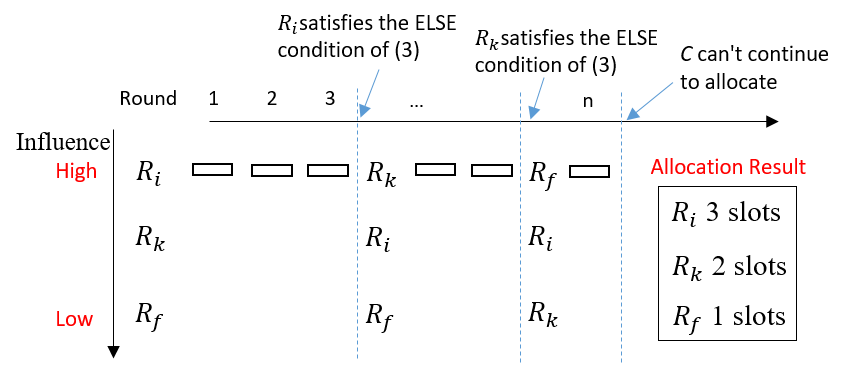
\includegraphics[width=8.5cm]{images/slot_allocation.png}
\label{fig_slot}

\caption{Slot allocation example}
\label{fig_model}
\end{figure}


\subsection{Co-Sampling slots ordering based on effectiveness maximizing greed}
In model (\ref{1}), we have described the effect of cooperative sampling between nodes on sampling accuracy and the effective ratio of sampling. As shown in Fig.(\ref{fig_1_model}), the cooperation in time dimension between nodes is reflected in the order of sampling Slots of each node.Two nodes covering same flows should be avoided sampling in the same slot.They should be arranged with the appropriate sampling order and cooperate with each other to maximize the effectiveness of the entire sampling system during period T.For this sub-problem, formula (\ref{minrpt}) is its optimization model. The optimization goal of the model is to minimize the number of resampled flows under given the number of Slots of each node.For any two sampling points $R_i, R_j$, assuming that $S_i, S_j$ are their Slot sets respectively, then $|S_i \bigcap S_j|$ indicates the number of times they are sampled under the same Slot;$|F_i^c \bigcap F_j^c|$ indicates the number of flows that thet cover the same.Therefore, the number of flows that are resampled between two nodes can be expressed as: $|S_i \bigcap S_j| \cdot |F_i^c \bigcap F_j^c|$.How to reasonably arrange the sampling time slot sequence of each node in the period T, so that the number of resampled flows of the whole system is minimized, thereby ensuring the minimum sampling packet repetition rate, so that the effectiveness of the whole sampling system is maximized.
\vskip 0.1 cm
\begin{spacing}{0.5}
\begin{small}
\begin{equation}
\min \sum{(\left| \widetilde{{{S}_{i}}}\bigcap \widetilde{{{S}_{j}}} \right|}\cdot \left| \widetilde{{{F}_{i}}}\bigcap \widetilde{{{F}_{j}}} \right|),\forall i,j\wedge j>i
\label{minrpt}
\end{equation}
\end{small}
\end{spacing}
\vskip 0.15 cm
This problem can be solved by using the search backtracking method, but it is a problem that cannot be solved in a polynomial time. Therefore, we consider a simple greedy algorithm to solve the approximate optimal solution of the problem.Algorithm 3 gives a description of the process.The $CNT$ array has been calculated in the previous section, indicating the number of slots for each node.At the beginning of the algorithm, initialize the $M^{slot}$ two-dimensional array to store the placement relationship between $R_i$ and $s^l$: $M^{slot}[i][l]=1$, which represents $R_i$ node sampling at $s^l$.In each round, an idle slot is selected for all nodes of $\forall i, CNT[i]\neq 0$, and the selected slot makes the number of resampled flows of the whole system the least compared to other optional slots.Through each round, the nodes greedily chooses a slot that minimizes the current the number of resampled flows of the entire system, when $i, CNT[0]=0$, the slots order of each node are selected, an approximate optimal solution is obtained.The time complexity of the algorithm is $O(L^2 \cdot K)$.Fig.6 demonstrates the process.In the example, the approximate solution we solved by this algorithm is 6 and the optimal solution is 5.
\begin{algorithm}[h]
\caption{Order of Time Slot Based on Greedy}
\begin{algorithmic}[1]
\REQUIRE  $M$ ~, $S$ ~, $c_j$
\WHILE{$CNT[i] > 0,\exists i \wedge i = 1,2...,k$}
\FOR{$i=1$; $i <= K$; $i++$}
\IF{$CNT[i] > 0$}
\STATE $Min = Max$ $Integer$
\FOR{$l=1$; $l < \frac{T}{t}$; $l++$}
\IF{$M^{slot}[i][l] = 0$}
\STATE $temp = \sum^{K}_{j=1 \wedge j != i}(\left| \widetilde{{{F}_{i}}}\bigcap \widetilde{{{F}_{j}}} \right| \cdot M^{slot}[j][l]) + H[l] $
\IF{$temp < Min$}
\STATE $Min = temp$; $Sp = l$ 
\ENDIF
\ENDIF
\ENDFOR
\STATE$M^{slot}[i][Sp] = 1$; $ CNT[i]--$; $H[Sp] = Min$
\ENDIF
\ENDFOR
\ENDWHILE

\RETURN $M^{slot}$
\label{code:recentEnd}
\end{algorithmic}
\end{algorithm}

\begin{figure}[!hhhhhhhhhht]
\centering
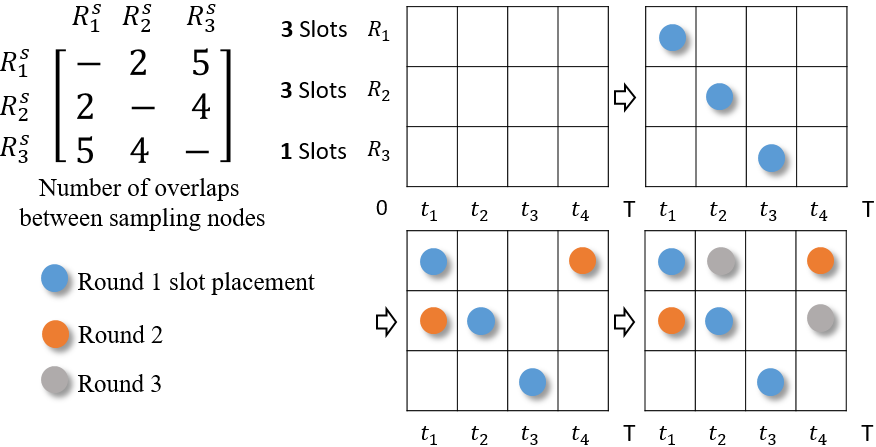
\includegraphics[width=7cm]{images/greedy_for_order_slot.png}
\caption{Illustrating sampling node slots placement based on greedy algorithm}
\label{slot_order}
\end{figure}

\section{Experiments and results}
In order to verify the effectiveness and performance of our algorithm, we have built a laboratory bed based on floodlight controller and openvswitch + mininet. The whole experimental bed contains 12 Dell XPS hosts, 20 core CPU, and Ubuntu 16.06.2 LTS. One runs a floodlight controller that fuses our algorithm, the other runs a data collector, and the remaining 10 deploy a network topology with 110 switch nodes and 50 host nodes. The experimental traffic dataset comes from the open project "the WIDE Project". We selected data from 14:00-14:15 in August 6, 2018. After cleaning and screening, we collate 5000 data streams for experiments. In the experiment, the number of data streams changed from 1000 to 5000..
We implement four algorithms: Random-K, top-K based on the extended median centrality, top-K based on the standard median centrality, our algorithm XXX. Based on the above four algorithms, we have made a comparative experiment in three measurement mechanisms: sampling accuracy, packet repetition rate and the number of rat streams collected.
Fig.x shows the comparison of sampling accuracy in different algorithms. Our algorithm is 7\% higher than Top-k and over 20\% than the other two algorithms. From Fig.x, we can see that different algorithms do almost the same amount of elephant flow collection. In fact, our algorithm only takes more part of the rat flow than other algorithms. And Fig.x shows that our algorithm is effective in reducing duplication and reducing it by more than 30\%.

\begin{figure}[!hhhhhhhhhht]
\centering
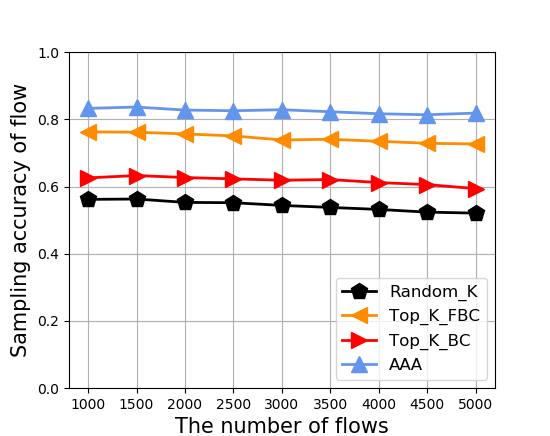
\includegraphics[width=7cm]{images/cmp_sam_accu.png}
\caption{accuracy comparison with respect to different algorithms}
\label{aaa.png}
\end{figure}
\begin{figure}[!hhhhhhhhhht]
\centering
\includegraphics[width=7cm]{images/cmp_rep_rate.png}
\caption{repetition rate comparison with respect to different algorithms}
\label{aaa.png}
\end{figure}

%\begin{figure}[!hhhhhhhhhht]
%\centering
%\includegraphics[width=8cm]{images/cmp_rep_rate.png}
%\caption{repetition rate comparison with respect to different algorithms }
%\label{aaa.png}
%\end{figure}

%\begin{figure}[!!!!!!!!!!!!!!hhhhhhhhhht]
%\centering
%\subfigure[ comparison of sampling accuracy]
%{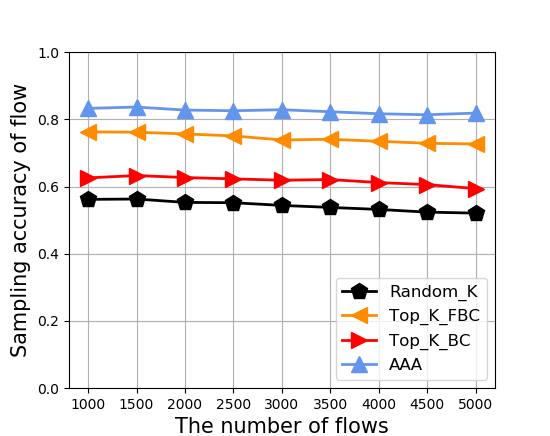
\includegraphics[width=4.1cm]{images/cmp_sam_accu.png}
%\label{fig_x_accu}
%}
%\subfigure[comparison of repetition rate]
%{\includegraphics[width=4.1cm]{images//cmp_rep_rate.png}
%\label{fig_x_rep}
%}
%\caption{comparison with respect to different algorithms}
%\label{fig_x_cmp}
%\end{figure}

\begin{figure}[!hhhhhhhhhht]
\centering
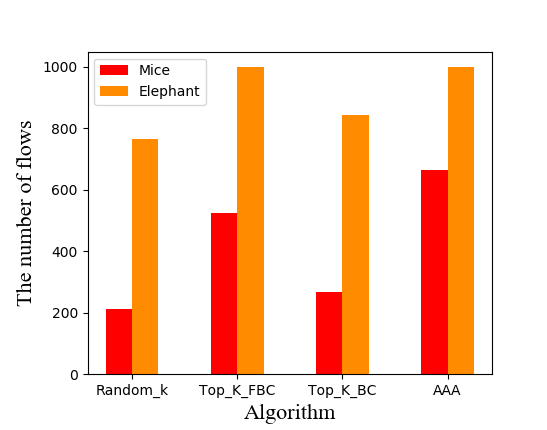
\includegraphics[width=8cm]{images/cmp_mice_flownum.png}
\caption{comparison of different algorithms in number of mice flow}
\label{aaa.png}
\end{figure}

\begin{figure}[!hhhhhhhhhht]
\centering
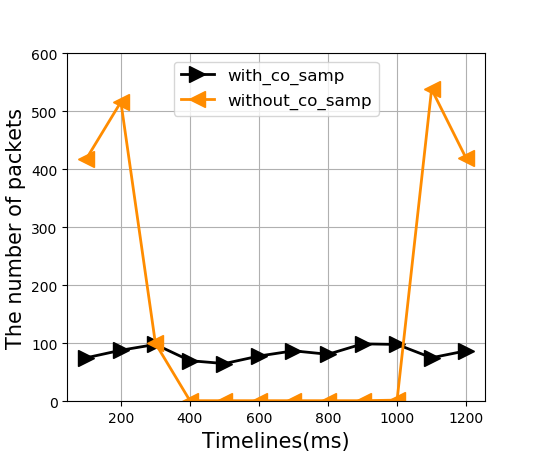
\includegraphics[width=8cm]{images/num_slot.png}
\caption{comparison of sampling flow number at different slot}
\label{aaa.png}
\end{figure}



\section{Conclusion}
\begin{itemize}
\item Lab environment
\item Sampling accuracy comparison
\item Sampling repetition rate comparison
\item Greedy centrality algorithm experimental results
 
\item Deduplication rate algorithm comparison

\item Experimental comparison of adaptive co-sampling algorithm
\end{itemize}



%\section{Conclusion}

%\begin{itemize}
%\item[-] Case 1: $ \frac{1}{SW_{num}} < S_{rate} \Leftrightarrow Confliction $   \\
%\item[-] Case 2: $ \frac{1}{SW_{num}} >= S_{rate} \Leftrightarrow no Confliction $ 


 





% trigger a \newpage just before the given reference
% number - used to balance the columns on the last page
% adjust value as needed - may need to be readjusted if
% the document is modified later
%\IEEEtriggeratref{8}
% The "triggered" command can be changed if desired:
%\IEEEtriggercmd{\enlargethispage{-5in}}

% references section

% can use a bibliography generated by BibTeX as a .bbl file
% BibTeX documentation can be easily obtained at:
% http://mirror.ctan.org/biblio/bibtex/contrib/doc/
% The IEEEtran BibTeX style support page is at:
% http://www.michaelshell.org/tex/ieeetran/bibtex/
%\bibliographystyle{IEEEtran}
% argument is your BibTeX string definitions and bibliography database(s)
%\bibliography{IEEEabrv,../bib/paper}
%
% <OR> manually copy in the resultant .bbl file
% set second argument of \begin to the number of references
% (used to reserve space for the reference number labels box)
\begin{thebibliography}{1}

\bibitem{1}
S.~Yoon, T.~Ha, S.~Kim and H.~Lim,\hskip 1em plus 0.5em minus 0.4em
Scalable Traffic Sampling using Centrality Measure on Software-Defined Networks, in \emph{IEEE Communications Magazine}, pp.43-49, July 2017.

\bibitem{1}
M.~Malboubi, L.~Wang, C.N.~Chuah, P.~Sharma,\hskip 1em plus 0.5em minus 0.4em
Intelligent SDN based Traffic (de)Aggregation and Measurement Paradigm (iSTAMP), in \emph{IEEE INFOCOM}, Apr 2014.

\bibitem{1}
L.~Tong and W.~Gao,\hskip 1em plus 0.5em minus 0.4em
Application-Aware Traffic Scheduling for Workload Offloading in Mobile Clouds, in \emph{IEEE INFOCOM}, pp.1-9, Apr 2016.

\bibitem{1}
J.~Jiang, S.~Ma, B.~Li and B.~Li,\hskip 1em plus 0.5em minus 0.4em
Symbiosis: Network-Aware Task Scheduling in Data-Parallel Frameworks, in \emph{IEEE INFOCOM}, pp.10-14, Apr 2016.

\bibitem{1}
P.~Bakopoulos, K.~Christodoulopoulos, G.~Landi et al,\hskip 1em plus 0.5em minus 0.4em
NEPHELE: An End-to-End Scalable and Dynamically Reconfgurable Optical Architecture for Application-Aware SDN Cloud Data Centers, in \emph{IEEE Communitions Magazine}, pp.178-188, Feb 2018.

\bibitem{2}
J.~Xu, J.Y.~Wang, Q.~Qi, H.F.~Sun and B.~He,\hskip 1em plus 0.5em minus 0.4em
IARA: An Intelligent Application-aware VNF for Network Resource Allocation with Deep Learning, in \emph{IEEE SECON}, pp.1-3, June 2018.

\bibitem{2}
J.~Suh, T.T.~Kwon, C.~Dixon, W.~Felter and J.~Carter,\hskip 1em plus 0.5em minus 0.4em
OpenSample: A Low-latency, Sampling-based Measurement Platform for Commodity SDN, in \emph{IEEE ICDCS}, pp.228-237, July 2014.

\bibitem{2}
Z.~Su, T.~Wang, Y.~Xia and M.~Hamdi,\hskip 1em plus 0.5em minus 0.4em
CeMon: A Cost-effective Flow Monitoring System in Software Defined Networks, in \emph{Computer Networks}, pp.101-115, Dec 2015.

\bibitem{3}
N.F.~Huang, C.C.~Li, C.H.~Li, C.C.~Chen,C.H.~C and I.H.~Hsu,\hskip 1em plus 0.5em minus 0.4em
Application Identification System or SDN QoS based on Machine Learning and DNS Responses, in \emph{APNOMS}, pp.407-410, Sept 2017.

\bibitem{3}
S.~Jeong, D.~Lee, J.~Hyun, J.~Li, and J.W.~Hong,\hskip 1em plus 0.5em minus 0.4em
Application-aware Traffic Engineering in Software-Defined Network, in \emph{APNOMS}, pp.315-318, Sept 2017.

\bibitem{3}
G.~Cheng and Y.~Tang,\hskip 1em plus 0.5em minus 0.4em
eOpenFlow: Software Defined Sampling via a Highly Adoptable OpenFlow Extension, in \emph{IEEE ICC}, pp.1-6, May 2017.


\bibitem{3}
S.~Zhao and D.~Medhi,\hskip 1em plus 0.5em minus 0.4em
Application Performance Optimization Using Application-Aware Networking, in \emph{IEEE NOMS},pp.1-6, Apr 2018.

\bibitem{4}
M.~Malboubi, S.M.~Peng, P.~Sharma and C.N.~Chuah,\hskip 1em plus 0.5em minus 0.4em
A Learning-based Measurement Framework for Traffic Matrix Inference in Software Defined Networks, in \emph{Computers \& Electrical Engineering}, Dec 2017.

\bibitem{4}
K.~Bilal, S.U.~Khan, L.~Zhang et al,\hskip 1em plus 0.5em minus 0.4em
Quantitative comparisons of the state-of-the-art data center architectures, in \emph{Concurrency \& Computation Practice \& Experience}, Dec 2017.

\end{thebibliography}




% that's all folks
\end{document}
